\documentclass{article}

\usepackage{arxiv}

\usepackage[utf8]{inputenc} % allow utf-8 input
\usepackage[T1]{fontenc}    % use 8-bit T1 fonts
\usepackage{hyperref}       % hyperlinks
\usepackage{url}            % simple URL typesetting
\usepackage{booktabs}       % professional-quality tables
\usepackage{amsfonts}       % blackboard math symbols
\usepackage{nicefrac}       % compact symbols for 1/2, etc.
\usepackage{microtype}      % microtypography
\usepackage{lipsum}		% Can be removed after putting your text content
\usepackage{graphicx}
\usepackage{doi}
\usepackage{xcolor}

\usepackage[backend=biber,sorting=none]{biblatex}
\addbibresource{references.bib}

\newcommand{\chioz}{\ensuremath{\widetilde{\chi}_{1}^{0}}}
\newcommand{\met}{\ensuremath{E_{\mathrm{T}}^{\mathrm{miss}}}}
\newcommand{\mapyde}{\texttt{mapyde}}
\newcommand{\simpleanalysis}{\texttt{SimpleAnalysis}}
\newcommand{\madgraph}{\textsc{MadGraph}}
\newcommand{\madspin}{\textsc{MadSPin}}
\newcommand{\pythia}{\textsc{Pythia}}
\newcommand{\delphes}{\textsc{Delphes}}
\newcommand{\pyhf}{\texttt{pyhf}}
\newcommand{\musig}{\ensuremath{\mu_{\mathrm{sig}}}}
\newcommand{\hepdata}{\texttt{HEPData}}

\title{Reduce, Reuse, Reinterpret: an end-to-end pipeline for reinterpreting particle physics results}

%\date{September 9, 1985}	% Here you can change the date presented in the paper title
%\date{} 					% Or removing it

\author{ \href{https://orcid.org/0000-0001-6616-3433}{
\includegraphics[scale=0.06]{orcid.pdf}\hspace{1mm}Giordon~Stark}\thanks{More information...} \\
  University of California, Santa Cruz \\
  Santa Cruz Institute for Particle Physics, \\
  Interdisciplinary Sciences Building, Room \#337, 1156 High Street \\
  Santa Cruz, CA 95064 \\
	\texttt{gistark@ucsc.edu} \\
	%% examples of more authors
	\and
	\href{https://orcid.org/0000-0001-8392-0934}{
\includegraphics[scale=0.06]{orcid.pdf}\hspace{1mm}Mike~Hance} \\
  University of California, Santa Cruz \\
  Santa Cruz Institute for Particle Physics, \\
  Natural Sciences 2, Room \#317, 1156 High Street \\
  Santa Cruz, CA 95064 \\
	\texttt{mhance@ucsc.edu} \\
	%% \AND
	%% Coauthor \\
	%% Affiliation \\
	%% Address \\
	%% \texttt{email} \\
	%% \and
	%% Coauthor \\
	%% Affiliation \\
	%% Address \\
	%% \texttt{email} \\
	%% \and
	%% Coauthor \\
	%% Affiliation \\
	%% Address \\
	%% \texttt{email} \\
}

% Uncomment to remove the date
%\date{}

% Uncomment to override  the `A preprint' in the header
%\renewcommand{\headeright}{Technical Report}
%\renewcommand{\undertitle}{Technical Report}
\renewcommand{\shorttitle}{\mapyde{} - an end-to-end pipeline workflow for particle physics}

%%% TODO
%%% Add PDF metadata to help others organize their library
%%% Once the PDF is generated, you can check the metadata with
%%% $ pdfinfo template.pdf
\hypersetup{
  pdftitle={mapyde - an end-to-end pipeline workflow for particle physics},
  pdfsubject={q-bio.NC, q-bio.QM},
  pdfauthor={Giordon~Stark, Mike~Hance},
  pdfkeywords={First keyword, Second keyword, More},
}

\begin{document}
\maketitle

\begin{abstract}
Searches for new physics at the Large Hadron Collider have constrained many models of physics beyond the Standard Model.  Many searches also provide resources that allow them to be reinterpreted in the context of other models.  We describe a reinterpretation pipeline that examines previously untested models of new physics using supplementary information from ATLAS SUSY searches, such as public analysis routines and serialized likelihoods, in a way that provides accurate limits even in models that differ meaningfully from the benchmark models of the original analysis .  These resources are combined with common event generation and simulation toolkits \madgraph, \pythia, and \delphes{} into workflows steered by \textsc{TOML} configuration files, and bundled into the \mapyde{} python package.  The use of \mapyde{} is demonstrated by constraining SUSY models with compressed sleptons and electroweakinos using ATLAS results.
\end{abstract}


%% %% keywords can be removed
%% \keywords{First keyword \and Second keyword \and More}


\section{Introduction}
\label{sec:introduction}

\begin{itemize}
\item Describe the reinterpretation problem.
\item Mention other toolkits:
  \begin{itemize}
  \item Full reinterpretation: RECAST
  \item Simplified likelihoods: GAMBIT? CHECKMATE?
  \item Others?
  \end{itemize}
\item Describe mapyde's approach
\item Paragraph describing this paper
\end{itemize}

\section{The \mapyde toolkit}
\label{sec:mapyde}

\begin{itemize}
\item Tools:
  \begin{itemize}
  \item General tools: Madgraph, Pythia, Delphes
  \item ATLAS tools: SA
  \item Fits: pyhf
  \end{itemize}
\item Configuration: TOML files
\item Runtime:
  \begin{itemize}
  \item Docker containers
  \item Python steering
  \end{itemize}
\item Outputs
\end{itemize}

\section{Reinterpreting Compressed SUSY Searches from ATLAS}
\label{sec:reinterp}

We demonstrate the utility of the analysis chain described above by reproducing and reinterpreting the results of ATLAS searches for supersymmetry.  The searches described in Ref.~\cite{ATLAS:2019lng} are optimized for SUSY models with ``compressed'' mass spectra, where the next-to-lightest SUSY partner (NLSP) and lightest SUSY partner (LSP) are separated by $\mathcal{O}(1-10)$ GeV in mass.  The small mass splittings imply low-momentum (soft) Standard Model decay products, since most of the momentum of the NLSP is given to the LSP.  The ATLAS searches focus on final states including two low-momentum (``soft'') charged leptons, substantial missing transverse momentum (\met) from the invisible LSP's (which in this case are the lightest neutralinos, \chioz), and one or more energetic jets that boost the SUSY system.  We focus specifically on two searches from that paper: a search optimized for light sleptons, and a search optimized for light electroweakinos, the SUSY partners of the SM electroweak bosons.

\subsection{Implementation}
\label{sec:reinterp-imp}

We use \mapyde to generate, shower, and simulate SUSY events, to analyze them using \simpleanalysis, and to interpret the results using \pyhf.  The implementation corresponds to \mapyde{} version \textcolor{red}{xxx, need to update to latest version and confirm it still runs}, with configuration cards and scripts provided in a public github repository~\cite{mapyde-user} (\textcolor{red}{need to fix up that area if Giordon hasn't done it already}).  The configuration uses \madgraph{} version 2.9.3, \pythia{} version 8.306, and \delphes{} version 3.5.0.  The \simpleanalysis{} code runs on dedicated containers provided by ATLAS~\cite{SAGitLabRegistry}, where we use the ``\texttt{EwkCompressed2018}'' selection corresponding to the analyses from~\cite{ATLAS:2019lng}.  The \mapyde{} package includes resources to convert the \delphes{} ROOT output into inputs for \simpleanalysis{} (\texttt{delphes2SA}) and from \simpleanalysis{} ROOT file outputs to JSON format (\texttt{SA2JSON}) used as input for \pyhf.  We use \pyhf{} version \textcolor{red}{xxx (need to figure out what we're running in \texttt{pyplotting})} to patch the public likelihoods provided in the \hepdata~\cite{HepData} repository for Ref.~\cite{ATLAS:2019lng} with the signal yields from \mapyde, and to compute upper limits on the signal strength, \musig.  When reproducing the results for the same benchmark models from Ref.~\cite{ATLAS:2019lng} the \pyhf{} output is compared with limit contours provided in \hepdata.

The signal samples produced in our \mapyde{} workflow differ from those used in Ref.~\cite{ATLAS:2019lng} in three significant ways.  First, events in the ATLAS samples contained either one or two jets in the matrix element in addition to a pair of SUSY particles, with the one- and $\geq$ two-jet processes merged in the parton shower using the CKKW-L algorithm.  In our setup, we produce only one-jet events in \madgraph, and allow \pythia{} to model the contributions from additional emissions.  Second, the ATLAS samples use \madspin{} to perform the three-body decays of the electroweakinos to SM leptons and a \chioz, while we perform decays using \pythia.  Third, and most importantly, the ATLAS samples use ATLAS simulation and reconstruction software to transform the \pythia{} output into ROOT files containing physics objects, while we use \delphes.

\textcolor{red}{Acceptance, efficiency, per-lepton efficiencies in the delphes card.}

\subsection{Compressed Sleptons}
\label{reinterp-slep}

\begin{itemize}
\item Cross sections, k-factors
\item Acceptance checks
\item Reproducing ATLAS results

\begin{figure}
  \centering
  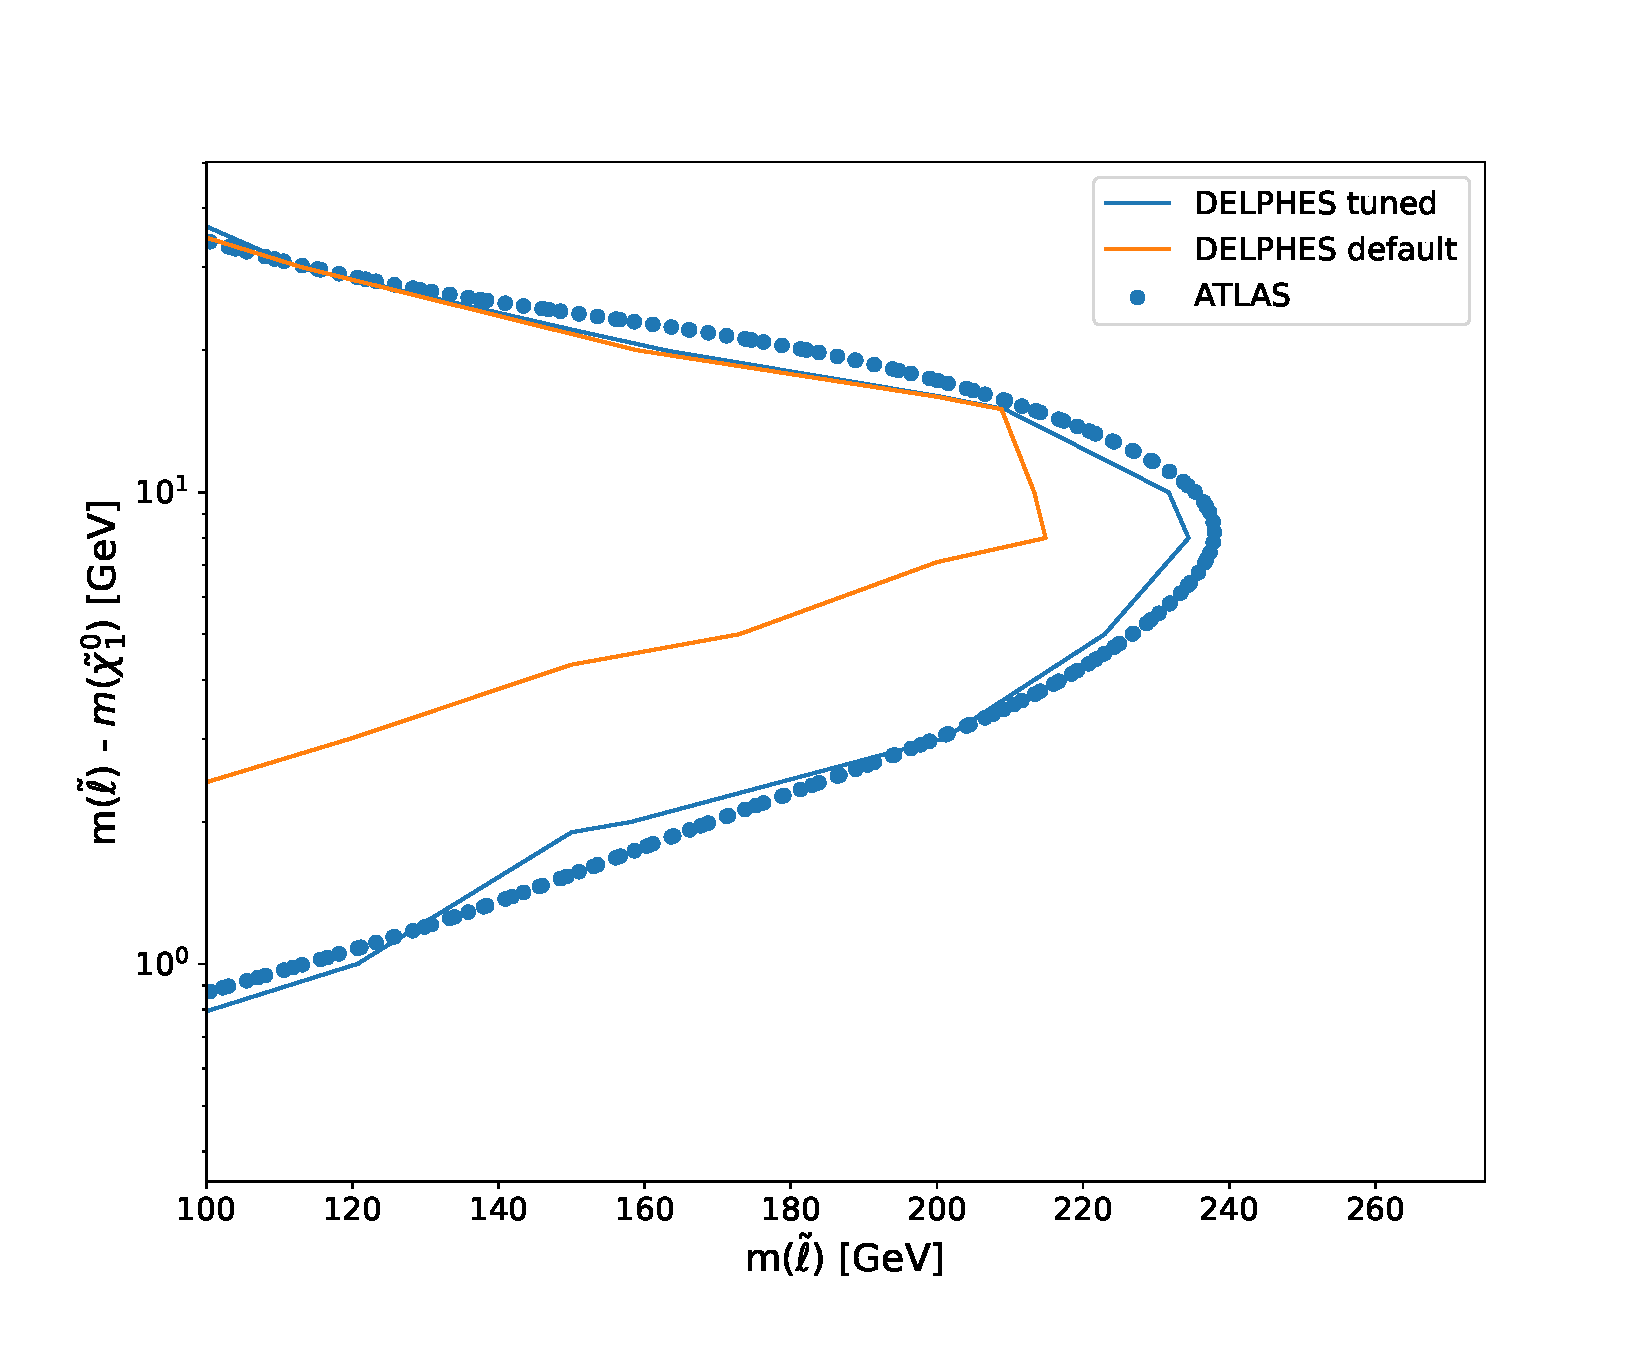
\includegraphics[width=0.8\textwidth]{{./figures/SleptonBino}}         %% examples/mapyde/SleptonBino_contours.ipynb
  \caption{Slepton limits}
  \label{fig:SleptonBino}
\end{figure}

\item Describing the slepton-wino-bino model

\begin{figure}
  \centering
  \includegraphics[width=0.5\textwidth]{{./figures/feynman/output/slepton_wino_bino}}
  \caption{Feynman Diagram of Slepton-Wino-Bino.}
  \label{fig:feynman:slepton_wino_bino}
\end{figure}

\item Results
\end{itemize}

\begin{figure}
  \centering
  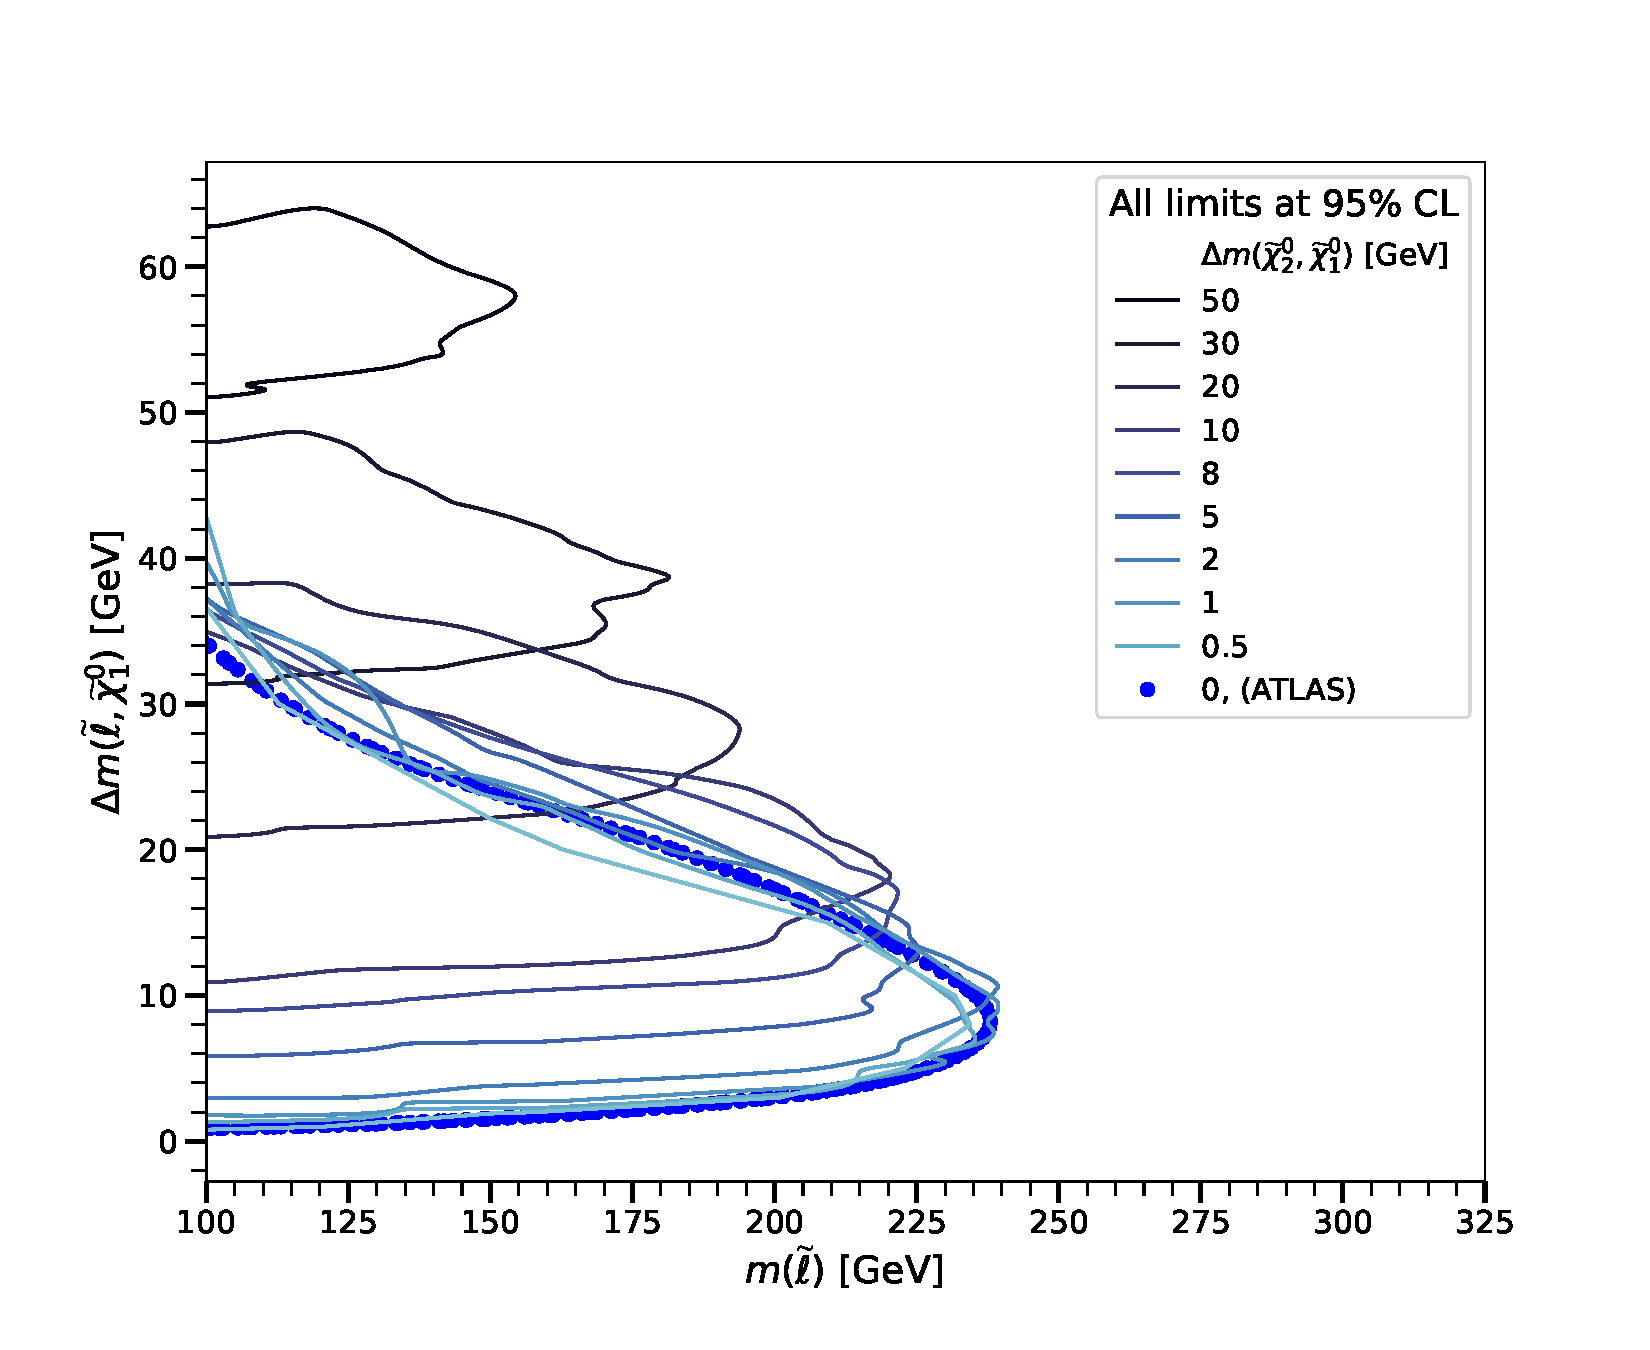
\includegraphics[width=0.48\textwidth]{{./figures/SleptonWinoBino_exp}}     %% examples/mapyde/SleptonWinoBino_contours.ipynb
  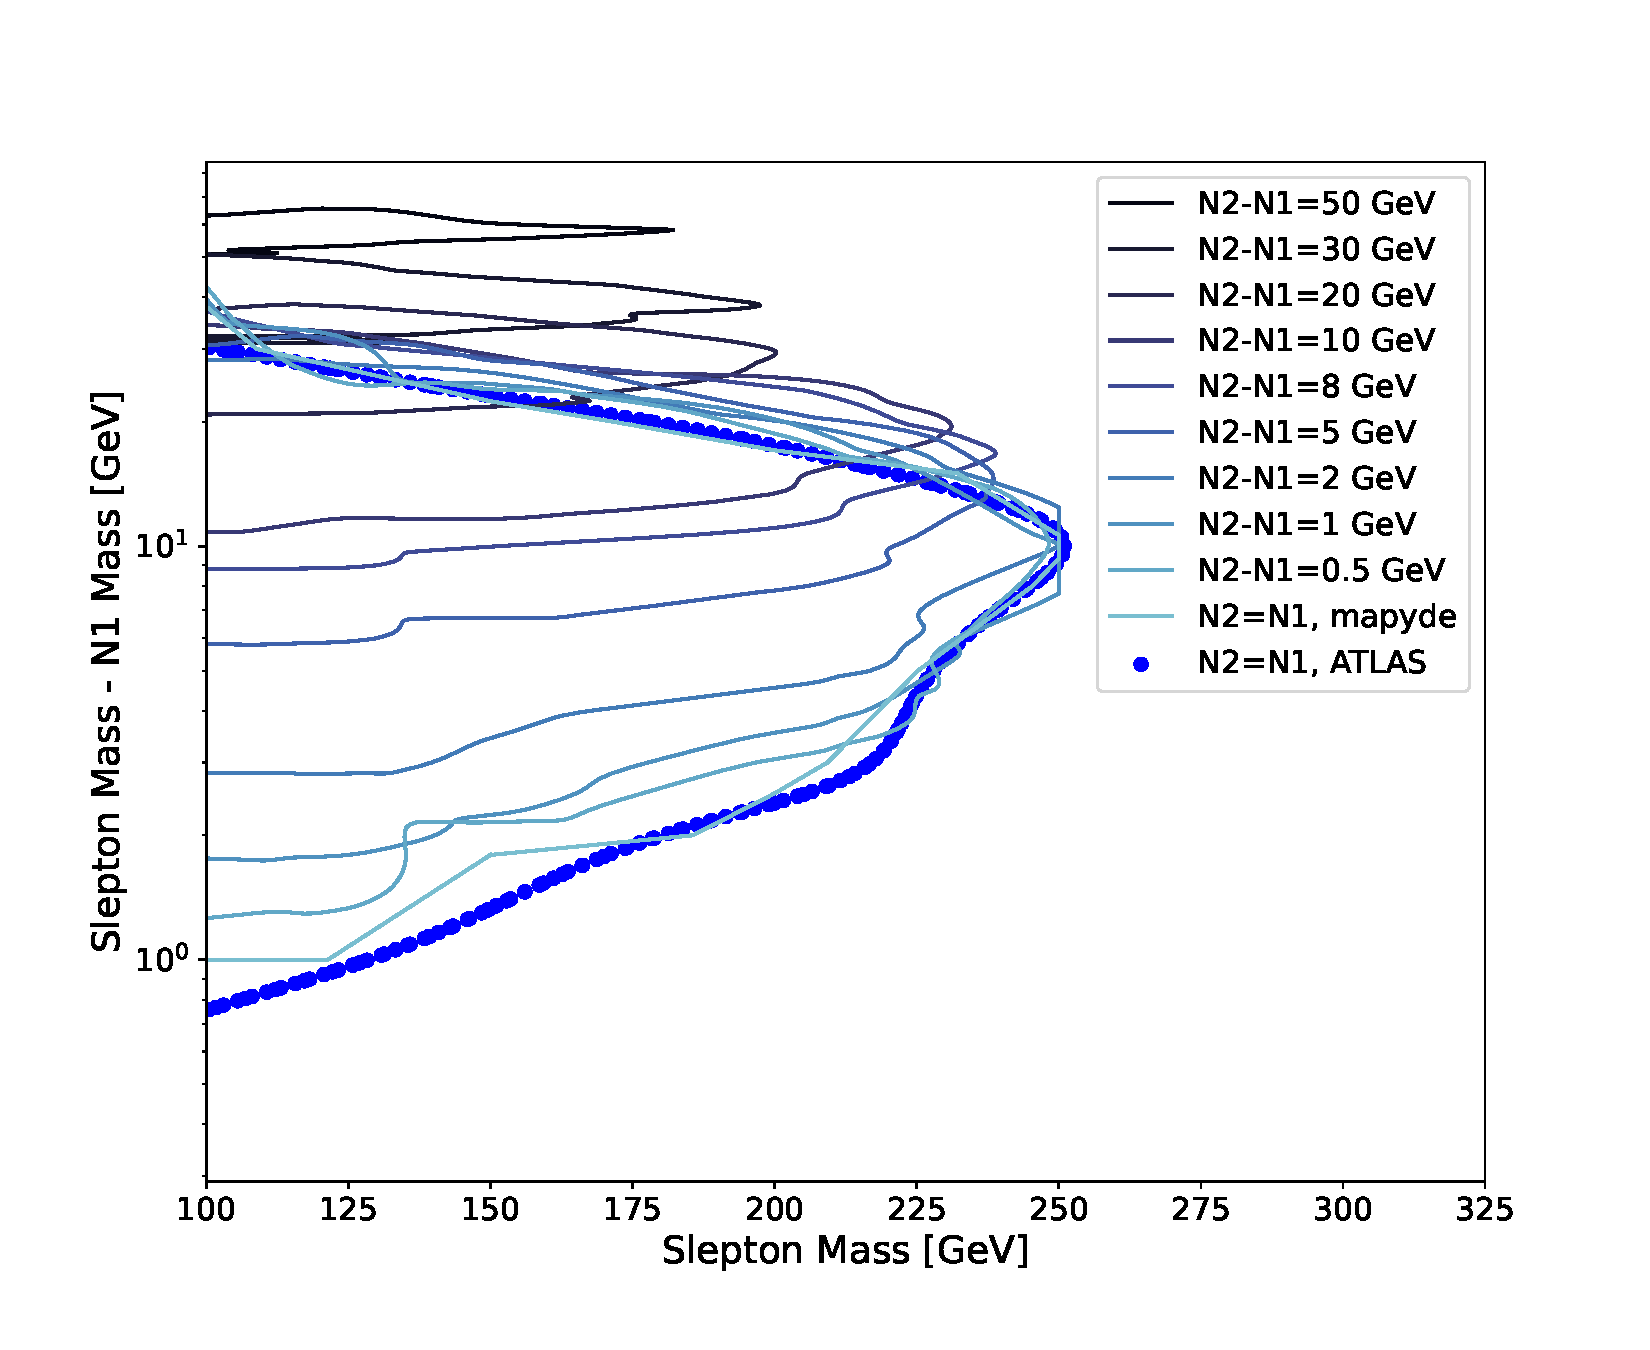
\includegraphics[width=0.48\textwidth]{{./figures/SleptonWinoBino_obs}}     %% examples/mapyde/SleptonWinoBino_contours.ipynb
  \caption{Slepton-Wino-Bino limits}
  \label{fig:SleptonWinoBino}
\end{figure}


\subsection{Compressed Electroweakinos}
\label{reinterp-ewkino}

\begin{itemize}
\item Reproducing ATLAS results

  \begin{figure}
  \centering
  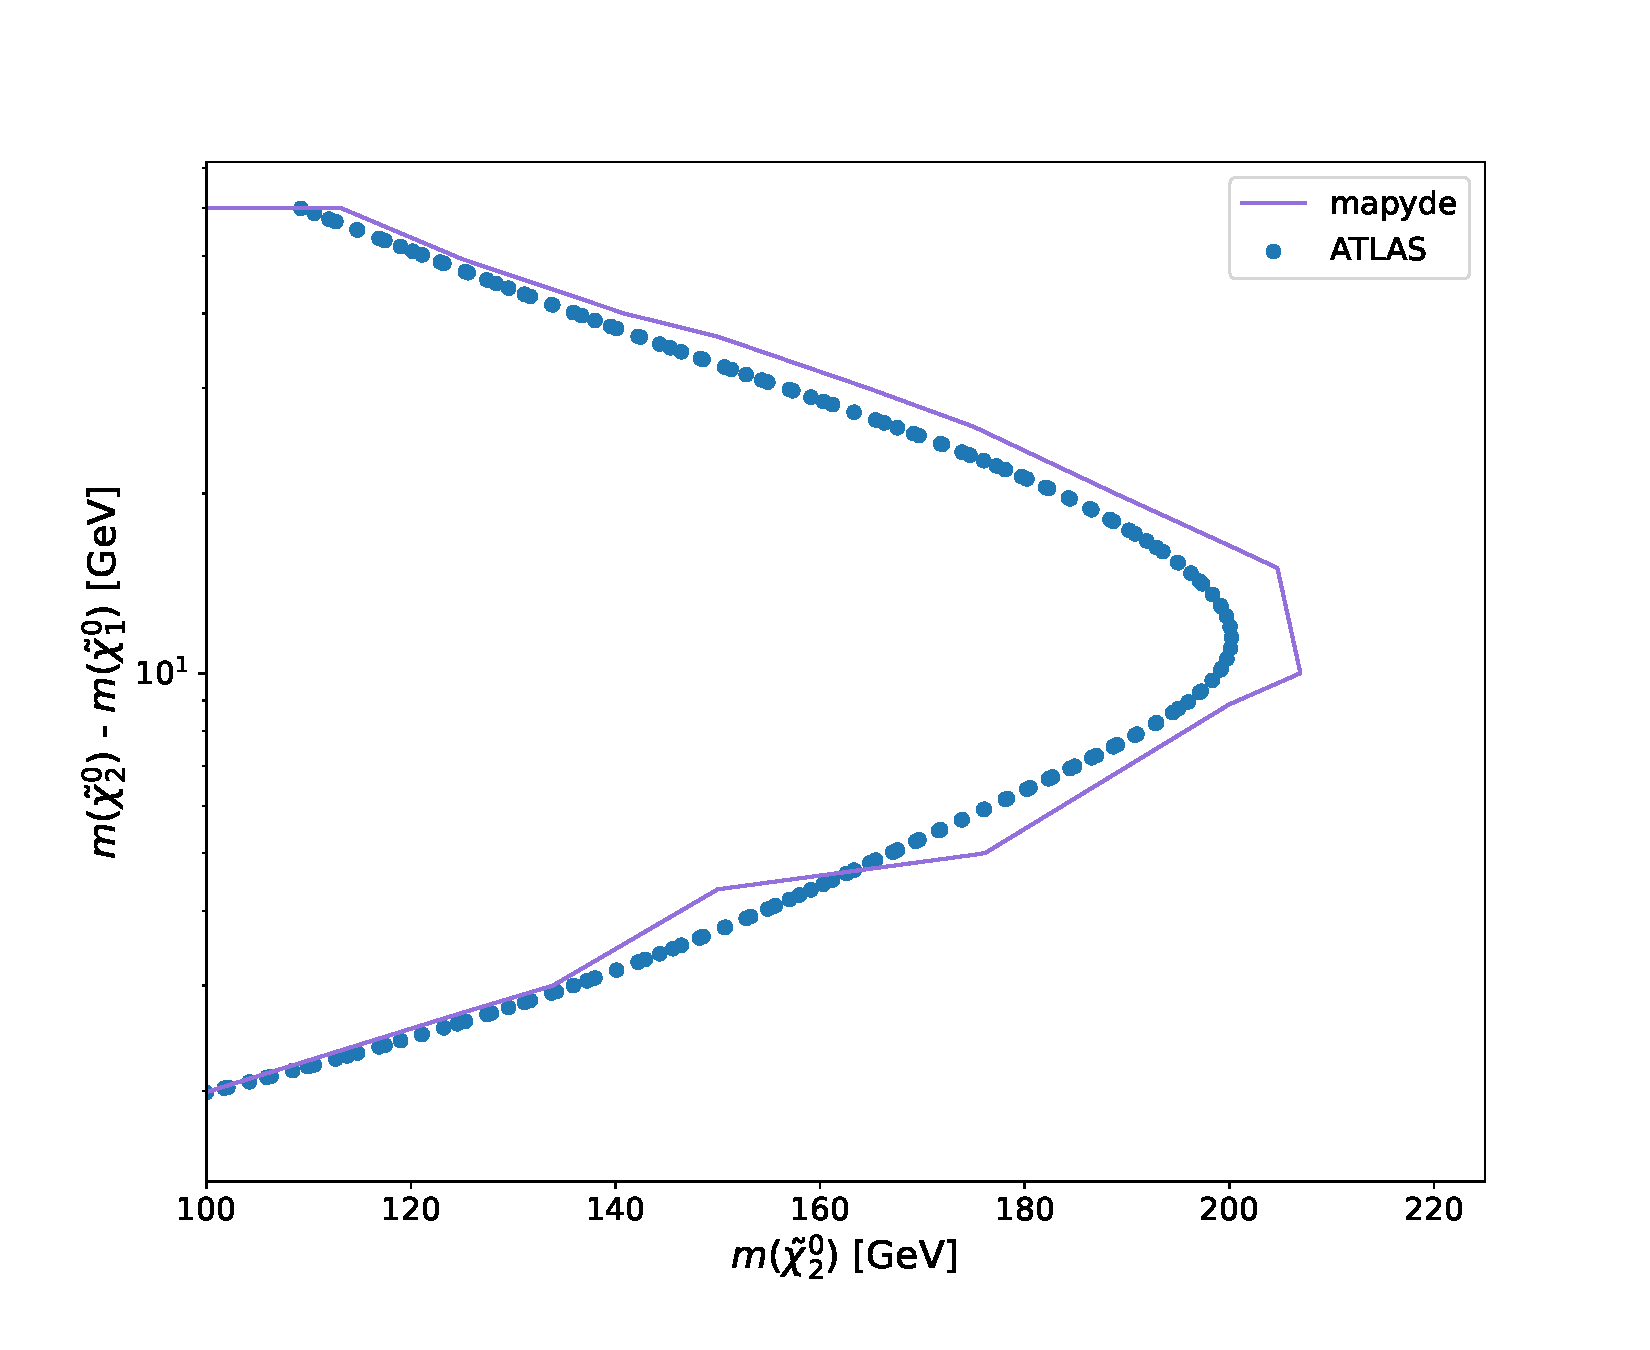
\includegraphics[width=0.8\textwidth]{{./figures/Higgsino}}         %% examples/mapyde/EWKino_contours.ipynb
  \caption{Higgsino limits}
  \label{fig:Higgsino}
\end{figure}

\item Describing the higgsino-wino-bino model
\item Results
\end{itemize}

\begin{figure}
  \centering
  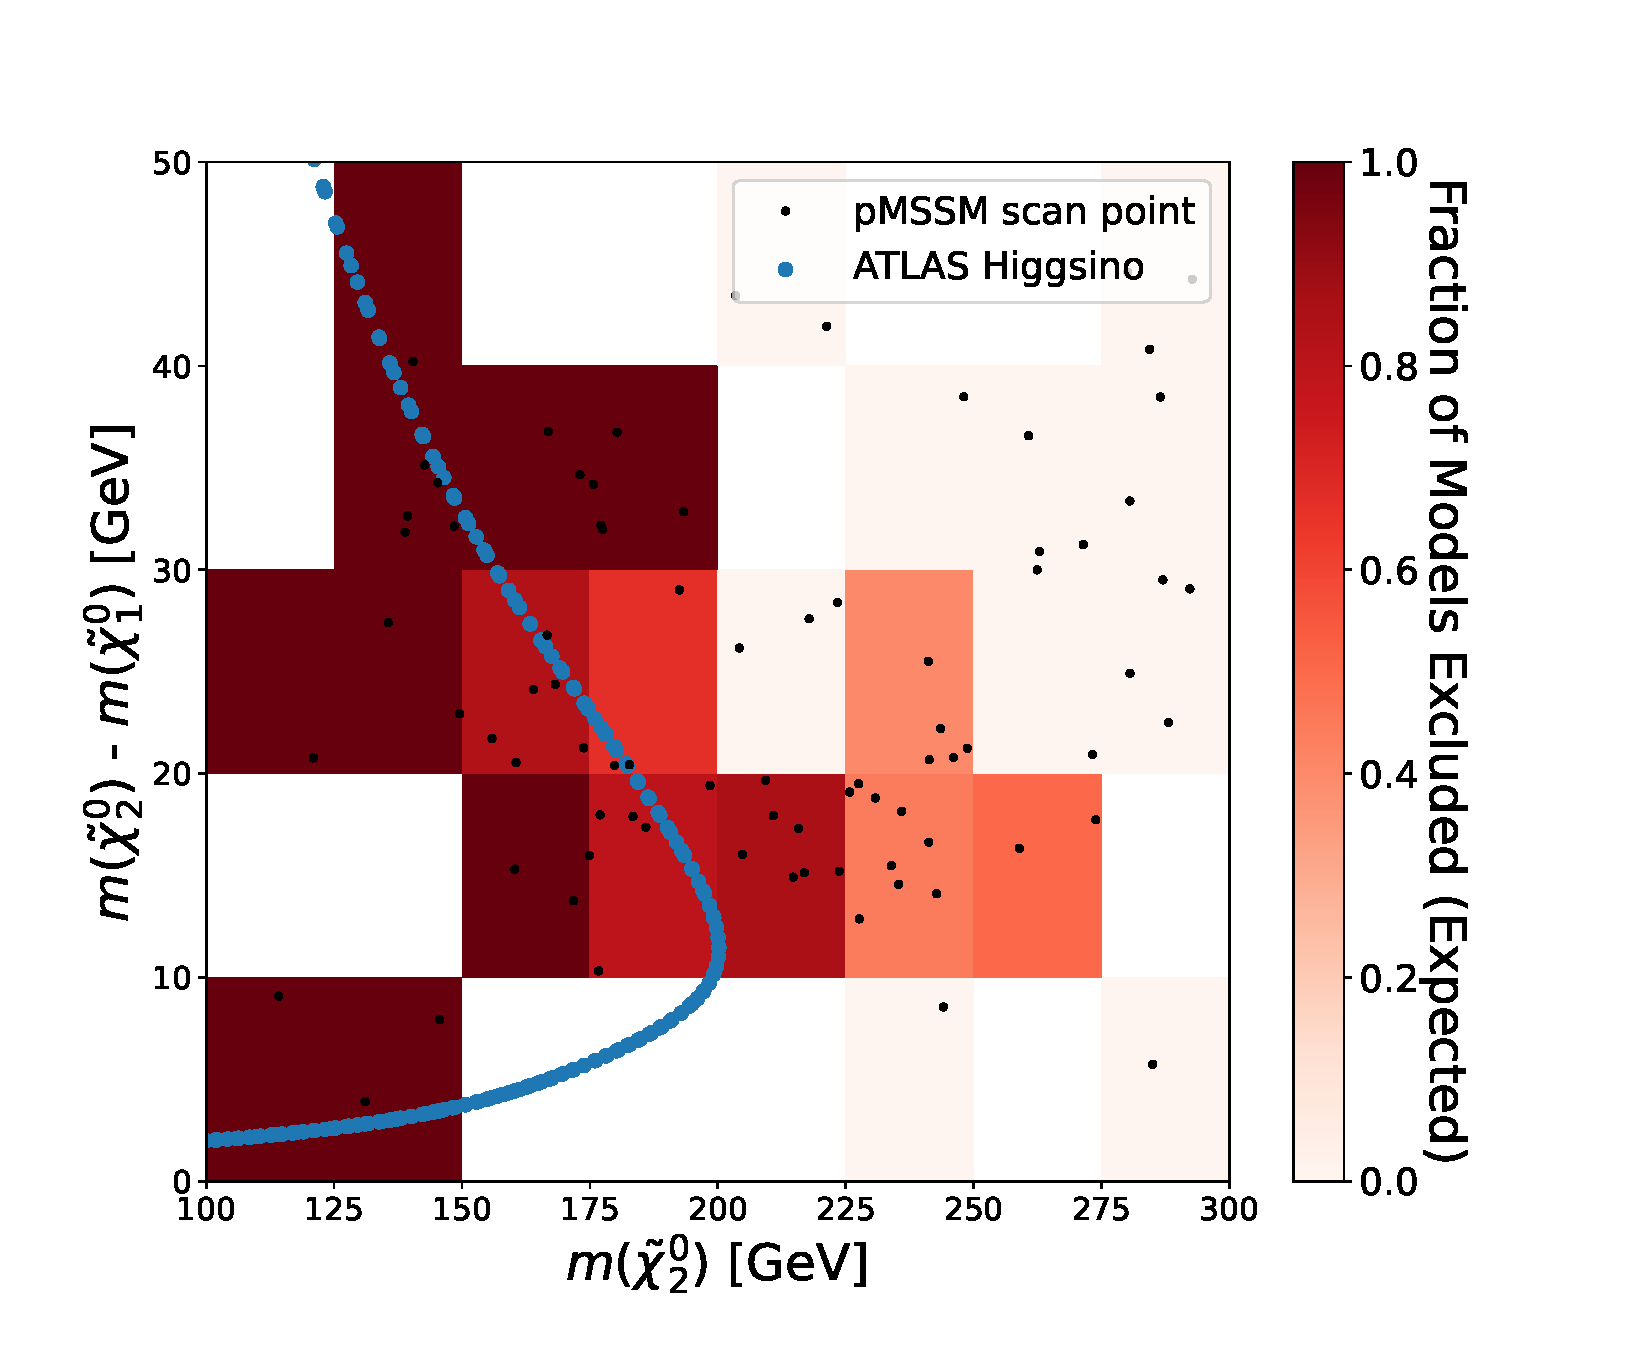
\includegraphics[width=0.48\textwidth]{{./figures/EWKino_pmssm_exp}}   %% examples/mapyde/WinoHiggsino_pmssm_contours.ipynb
  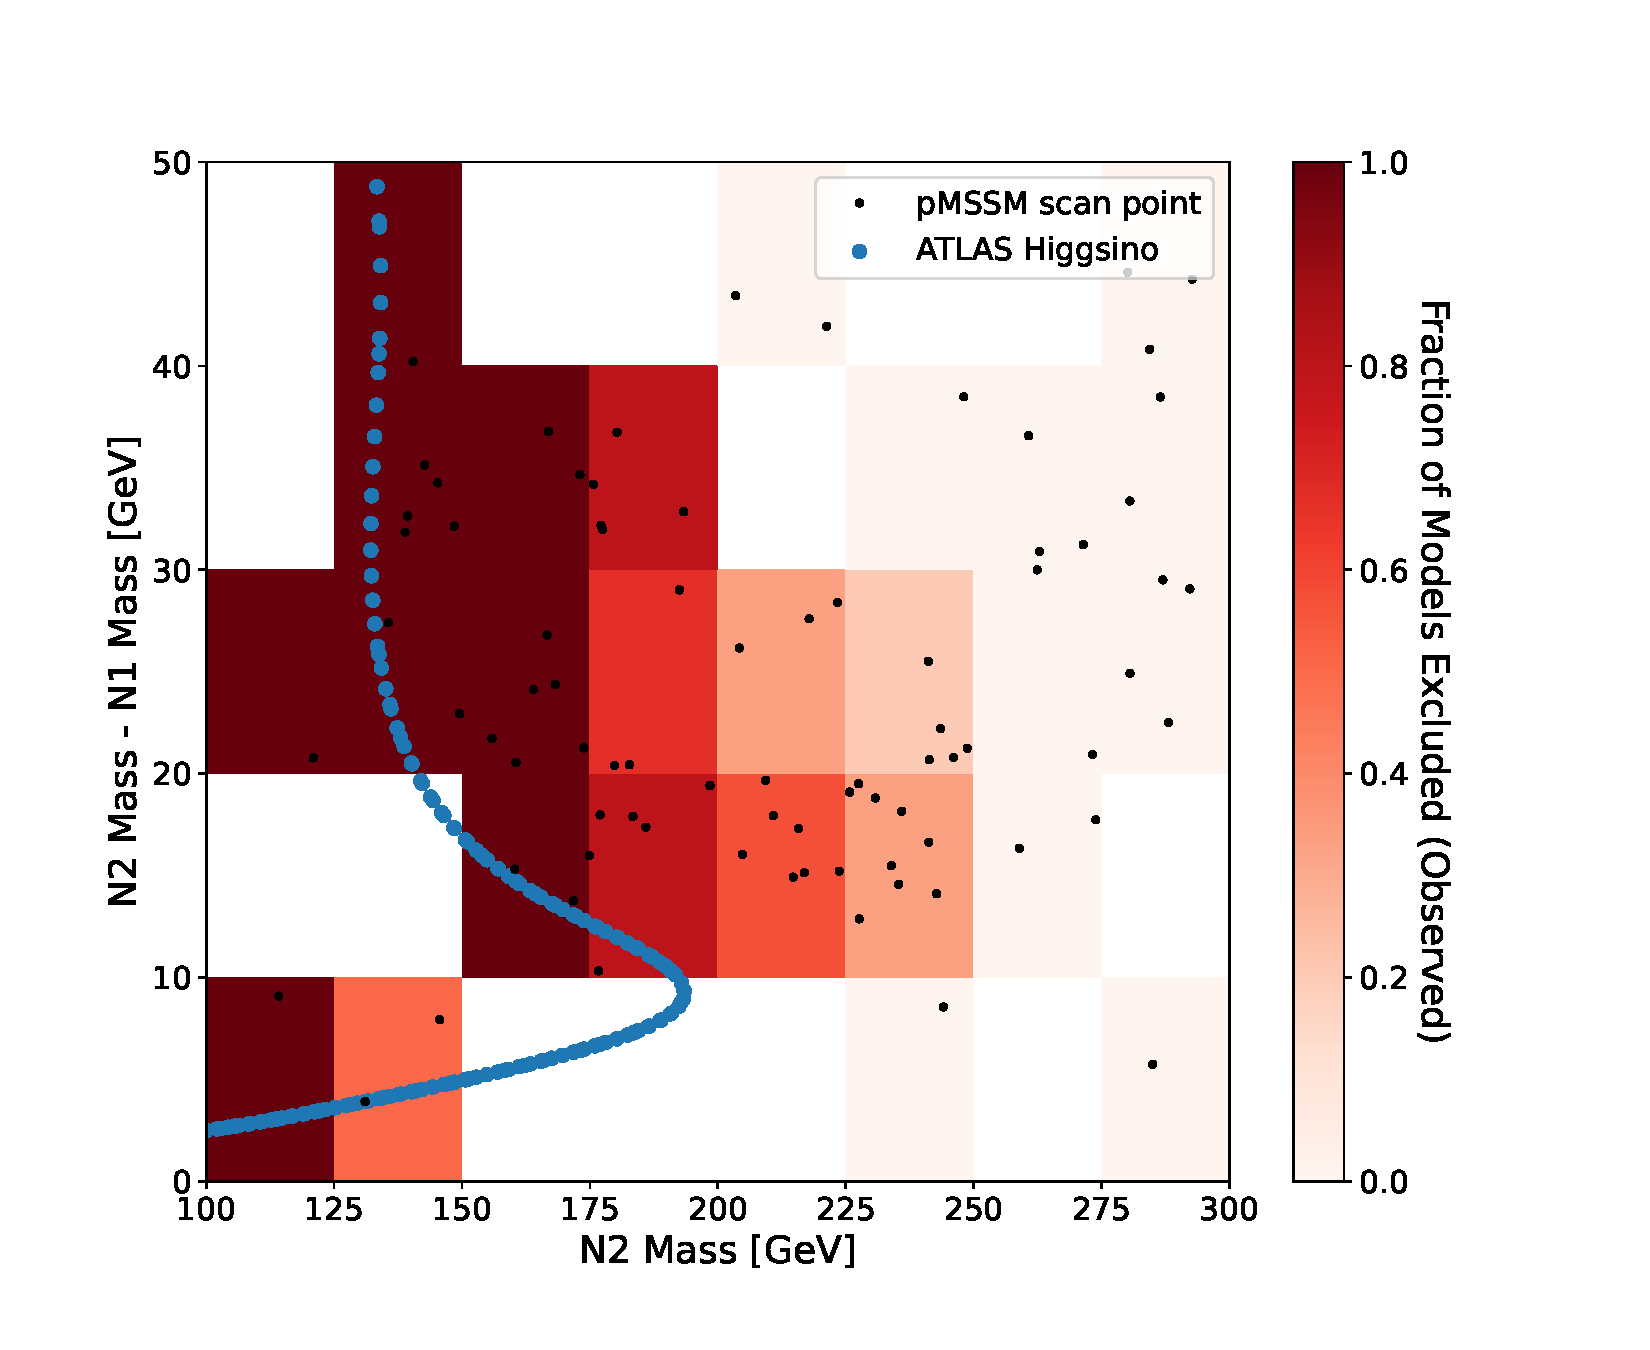
\includegraphics[width=0.48\textwidth]{{./figures/EWKino_pmssm_obs}}   %% examples/mapyde/WinoHiggsino_pmssm_contours.ipynb
  \caption{Higgsino-Wino-Bino limits}
  \label{fig:EWKino_pmssm}
\end{figure}

\section{Conclusion}

We have presented \texttt{mapyde}, shown some reinterpretations, and we're done.

\printbibliography

\end{document}
